\documentclass[tikz]{standalone}
\usetikzlibrary{positioning}

\begin{document}
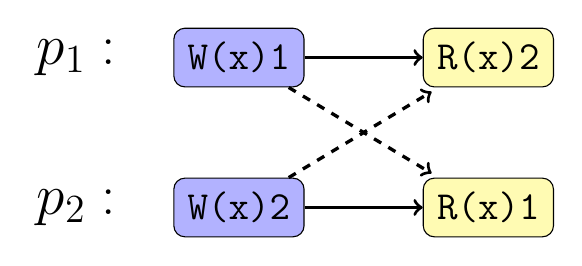
\begin{tikzpicture}
\tikzset{
  wop/.style = {rectangle, rounded corners, fill = blue!30, draw, font = \Large, inner sep = 5pt},
  rop/.style = {rectangle, rounded corners, fill = yellow!30, draw, font = \Large, inner sep = 5pt}, process/.style = {font = \huge}, po/.style = {->, very thick},
  rw/.style = {->, shorten >= 3pt, very thick, dashed},
  vis/.style = {->, shorten >= 3pt, very thick, dashed}
}

  \node (p1) [process] {$p_1:$};
  \node (wx1) [wop, right = 0.6cm of p1] {\texttt{W(x)1}};
  \node (rx2) [rop, right = 1.5cm of wx1] {\texttt{R(x)2}};

  \node (p2) [process, below = 1.2cm of p1] {$p_2:$};
  \node (wx2) [wop, right = 0.6cm of p2] {\texttt{W(x)2}};
  \node (rx1) [rop, right = 1.5cm of wx2] {\texttt{R(x)1}};

  \draw [po] (wx1) to (rx2);
  \draw [po] (wx2) to (rx1);

  \draw [vis] (wx1) to (rx1);
  \draw [vis] (wx2) to (rx2);
  %\draw [rw] (wx1) to [out = 0, in = 100] (rx1p3);

%  \node (p1-serial) [font = \huge, below right = 2.0cm and 3.0cm of p3] {$p_1:$ \texttt{W(x)0, W(x)1, W(y)2, W(y)3}};

\end{tikzpicture}
\end{document}